\documentclass[border=10pt]{standalone}
\usepackage{tikz}
\usepackage{amsmath}
\definecolor{myred}{RGB}{190,60,45}
\begin{document}
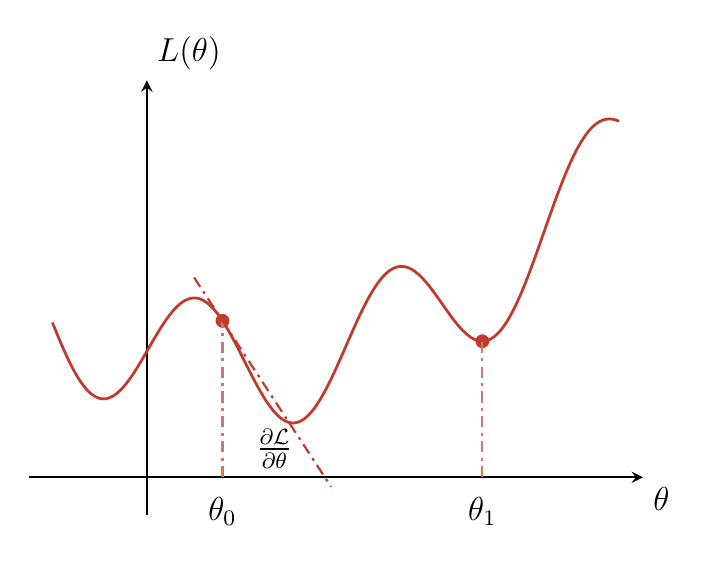
\begin{tikzpicture}[x=0.6cm, y=0.8cm, >=stealth, line width=0.8pt, font=\large]
  % f(x)  = sin(1.5x) + 0.05x^2 - 0.2x + 2
  % f'(x) = 1.5cos(1.5x) + 0.1x - 0.2
  \pgfmathsetmacro{\xt}{1.6}    % 切点 θ₀
  \pgfmathsetmacro{\yt}{sin(deg(1.5*\xt)) + 0.05*\xt*\xt - 0.2*\xt + 2}
  \pgfmathsetmacro{\mt}{1.5*cos(deg(1.5*\xt)) + 0.1*\xt - 0.2}
  \pgfmathsetmacro{\xo}{7.1}    % 右侧局部极小 θ₁（f'=0 处）
  \pgfmathsetmacro{\yo}{sin(deg(1.5*\xo)) + 0.05*\xo*\xo - 0.2*\xo + 2}

  % 坐标轴
  \draw[->] (-2.5,0) -- (10.5,0) node[below right] {$\theta$};
  \draw[->] (0,-0.6) -- (0,6.3)  node[above right] {$L(\theta)$};

  % 损失曲线
  \draw[myred, line width=1pt, domain=-2:10, samples=200]
        plot (\x, {sin(deg(1.5*\x)) + 0.05*\x*\x - 0.2*\x + 2});

  % θ₀：切点 + 竖直点划线 + 真切线
  \fill[myred] (\xt,\yt) circle (2.5pt);
  \draw[myred!70, dash pattern=on 4pt off 2pt on 1pt off 2pt] (\xt,0) -- (\xt,\yt);
  \draw[myred, dash pattern=on 4pt off 2pt on 1pt off 2pt]
        ({\xt-0.6},{\yt-0.6*\mt}) -- ({\xt+2.3},{\yt+2.3*\mt});

  % θ₁：局部极小，竖直点划线落轴（新增）
  \fill[myred] (\xo,\yo) circle (2.5pt);
  \draw[myred!70, dash pattern=on 4pt off 2pt on 1pt off 2pt] (\xo,0) -- (\xo,\yo);

  % 标签
  \node[below] at (\xt,-0.15) {$\theta_0$};
  \node[below] at (\xo,-0.15) {$\theta_1$};
  \node[above] at (2.7,-0.03)   {$\frac{\partial \mathcal{L}}{\partial \theta}$};
\end{tikzpicture}
\end{document}